
\provideboolean{riskyAltYN}\setboolean{riskyAltYN}{false}\newcommand{\ifriskyAlt}{\ifthenelse{\boolean{riskyAltYN}}}
\newcommand{\scale}{x}
%\setboolean{riskyAltYN}{true}

\newcommand{\riskyshk}{\varepsilon}
\newcommand{\riskyshkvar}{\sigma^{2}_{\riskyshk}}

\cite{merton:restat} and \cite{samuelson:portfolio} study the optimal portfolio choice of a consumer with constant relative risk aversion $\CRRA$.\footnote{$\uFunc(\cRat) = (1-\CRRA)^{-1}\cRat^{1-\CRRA}$.}  At the end of period~$t$ this consumer has assets $a_{t}$, and is deciding how much to invest in a risky asset\footnote{Both papers present the solution in the case with multiple risky assets; for the two-asset case, see \handoutA{Portfolio-Multi-CRRA}.} with a lognormally distributed return factor $\Risky_{t+1}$ (its log return $\riskyELog_{t+1} = \log \Risky_{t+1}$ is distributed normally), $\riskyELog_{t+1} = \riskyELog+\riskyshk_{t+1} \sim \mathcal{N}(\riskyELog,\riskyshkvar)$ for $\riskyshk_{t+1}\sim\mathcal{N}(0,\riskyshkvar)$.  {\ELogNorm}~reviews the well-known fact that in such a case the expectation of the return in levels (the `arithmetic' mean; see \ArithmeticVSGeometric) is $\Ex_{t}[\Risky_{t+1}]=e^{\riskyELog+(1/2)\riskyshkvar}$ so that for small $\riskyELog$ and $\riskyshkvar$ we will have an excellent approximation: defining $\riskyELev=\riskyELog+(1/2)\riskyshkvar$, it will be true that $\Ex_{t}[\Risky_{t+1}] \approx 1 + \riskyELev$ (again see~{\ArithmeticVSGeometric}).  For the rest of this handout, we will usually treat this approximation as an exact relationship.\footnote{The reason we construct things this way is that we want to be able to consider the consequences of a pure increase in $\riskyshkvar$ that leaves the return the consumer cares about -- the arithmetic return -- unchanged.  That is accomplished by defining the problem's `primitives' as being the arithmetic return and $\riskyshkvar$, so that when we increase $\riskyshkvar$ and solve the problem with $\riskyELog = \riskyELev - \riskyshkvar/2$ we will achieve the same expected arithmetic return as before the increase in $\riskyshkvar$.}
\begin{equation}\begin{gathered}\begin{aligned}
    \ifriskyAlt{\log \Risky_{t+1} = \riskyELev_{t+1} = }{\log \Ex_{t}[\Risky_{t+1}]  }       & =  \overbrace{\riskyELog_{}+0.5\sigma^{2}_{\risky}}^{\equiv \riskyELev_{}}
    \\   & =  \underbrace{\riskyELev_{}-0.5\sigma^{2}_{\risky}}_{=\riskyELog_{}}
\end{aligned}\end{gathered}\end{equation}

Any $\aNrm_{t}$ NOT invested in the risky asset is assumed to be invested in a riskfree asset that earns return factor
  $\Rfree=e^{\rfree}$.  Importantly, the consumer is assumed to have
  no labor income and to face no risk aside from that caused by their investment in
  the risky asset.\footnote{A common interpretation is that this is
    the problem of a retired investor who expects to receive no
    further labor income.  Note however that {\it all} risks other
    than the returns from financial investments have been ruled out;
    for example, health expense risk is not possible in this model,
    though recent research has argued such risk is important (maybe even dominant) later in
    life (cf.\ \cite{aclvJoy}).}$^{,}$\footnote{Riskless labor income can trivially be added
    to the problem, because its risklessness means that (in the
    absence of liquidity constraints) it is indistinguishable from a
    lump sum of extra current wealth with a value equal to the present
    discounted value (using the riskless rate) of the (riskless)
    future labor income.  Of course, in practice, labor income is not
    riskless, but when labor income is risky the problem no longer has
    the tidy analytical solution described here and must be solved
    numerically.  See \cite{SolvingMicroDSOPs} for an introduction to
    numerical solution methods.}

Both papers consider a multiperiod optimization problem, but here we
examine a consumer for whom period $t$ is the
second-to-last period of life (the insights, and even the formulas,
carry over to the multiperiod case).\footnote{\cite{samuelson1979we}.}

If the period-$t$ consumer invests proportion $\riskyshare$ in the risky asset,
spending all available resources in the last period of life $t+1$ will yield:
\begin{equation}\begin{gathered}\begin{aligned}
        c_{t+1} & =  \left(\Rfree(1-\riskyshare)+\Risky_{t+1}\riskyshare\right)a_{t} \notag
\\ & =  \underbrace{\left(\Rfree+(\Risky_{t+1}-\Rfree)\riskyshare\right)}_{\equiv \Rport_{t+1}}a_{t} \label{eq:RportDef}
\end{aligned}\end{gathered}\end{equation}
where $\Rport_{t+1}$ is the realized arithmetic %\footnote{If (magically) the portfolio return is instead geometric $\Rfree^{1-\riskyshare}\Risky^{\riskyshare}$ -- magically because this is not how portfolio returns occur in the real world -- then the approximate formulas below become exact; economists sometimes assume geometric portfolio returns just to simplify the math.}
return factor for the portfolio.

The optimal portfolio share will be the one that maximizes expected utility:
\begin{equation}\begin{gathered}\begin{aligned}
  \varsigma & =  \argmax_{\varsigma} ~ \Ex_{t}[\uFunc(c_{t+1})]
\end{aligned}\end{gathered}\end{equation}
and can be calculated numerically for any arbitrary distribution of rates of return.

\cite{cvAppendix} show that if we define the `equity premium' as
\begin{equation}\begin{gathered}\begin{aligned}
  \EpremLog_{t+1} & =  \riskyELog_{t+1}-\rfree + (1/2)\sigma^{2}_{\risky} \label{eq:eprem}
\end{aligned}\end{gathered}\end{equation}
then for many distributions a good approximation to the portfolio rate of return (the log of the portfolio return factor) is obtained by\footnote{See the appendix for further details.}
\begin{equation}\begin{gathered}\begin{aligned}
  \rport_{t+1} & =  \rfree+ \riskyshare \EpremLog_{t+1}+\riskyshare \sigma^{2}_{\risky}/2 - \riskyshare^{2}\sigma^{2}_{\risky}/2 \label{eq:rportCV}.
\end{aligned}\end{gathered}\end{equation}

Using this approximation, the expectation as of date $t$ of utility at date $t+1$ is:\footnote{The tedious full derivation is:
  \begin{equation}\begin{split}
  \Ex_{t}[\uFunc(c_{t+1})] & \approx  (1-\CRRA)^{-1}\Ex_{t}\left[\left(a_{t}e^{\rfree}e^{\riskyshare \EpremLog_{t+1}+\riskyshare(1-\riskyshare)\sigma^{2}_{\risky}/2 }\right)^{1-\CRRA}\right] \notag
\\                      & \approx  (1-\CRRA)^{-1}\Ex_{t}\left[(a_{t}\Rfree)^{1-\CRRA}\left( e^{\riskyshare \EpremLog_{t+1}+\riskyshare(1-\riskyshare)\sigma^{2}_{\risky}/2 }\right)^{1-\CRRA}\right]
\\                      & \approx  (1-\CRRA)^{-1}(a_{t}\Rfree)^{1-\CRRA}\Ex_{t}\left[e^{(\riskyshare \EpremLog_{t+1}+\riskyshare(1-\riskyshare)\sigma^{2}_{\risky}/2)  (1-\CRRA)}\right]
\\                      & \approx  \underbrace{(1-\CRRA)^{-1}(a_{t}\Rfree)^{1-\CRRA}}_{\text{constant $< 0$}}\underbrace{e^{ (1-\CRRA)\riskyshare(1-\riskyshare)\sigma^{2}_{\risky}/2}\Ex_{t}\left[e^{\riskyshare \EpremLog_{t+1}  (1-\CRRA)}\right]}_{\text{excess return utility factor}}
 \end{split}
  \end{equation}
}
\begin{equation}\label{eq:exputil}\begin{split}
  \Ex_{t}[\uFunc(c_{t+1})] & \approx  \underbrace{(1-\CRRA)^{-1}(a_{t}\Rfree)^{1-\CRRA}}_{\text{constant $< 0$}}\underbrace{e^{ (1-\CRRA)\riskyshare(1-\riskyshare)\sigma^{2}_{\risky}/2}\Ex_{t}\left[e^{\riskyshare \EpremLog_{t+1}  (1-\CRRA)}\right]}_{\text{excess return utility factor}}
 \end{split}
  \end{equation}
where the first term is a negative constant under the usual assumption that relative risk aversion $\CRRA>1.$

\hypertarget{lognormal-returns}{}
For the special (but reasonable) case of a lognormally distributed return, we can make substantial further progress, by obtaining an analytical approximation to the numerical optimum.  In this case $\riskyshare (1-\CRRA) \EpremLog_{t+1} \sim \mathcal{N}(\riskyshare (1-\CRRA)(\EpremLog - \Evarr/2),(\riskyshare(1-\CRRA))^{2}\Evarr)$ (again using \LogELogNormTimes).  With a few extra lines of derivation we can show that the log of the expectation in \eqref{eq:exputil} is\footnote{Full derivation:
\begin{equation}\begin{split}
  \log \Ex_{t}\left[e^{\riskyshare \EpremLog_{t+1}  (1-\CRRA)}\right] & =  {(1-\CRRA)\riskyshare \EpremLog-(1-\CRRA)\riskyshare\Evarr/2+ ((1-\CRRA)\riskyshare)^{2}\Evarr/2} \notag
\\  & =  {(1-\CRRA)\riskyshare \EpremLog-(1-\CRRA)\riskyshare(1-\riskyshare(1-\CRRA))\Evarr/2}
\\  & =  {(1-\CRRA)\riskyshare \EpremLog-(1-\CRRA)\riskyshare(1-\riskyshare)\Evarr/2-\CRRA (1-\CRRA)\riskyshare^{2}\Evarr/2}.
\end{split}\end{equation}
}
\begin{equation}\label{eq:Ex}\begin{split}
  \log \Ex_{t}\left[e^{\riskyshare \EpremLog_{t+1}  (1-\CRRA)}\right] & =  {(1-\CRRA)\riskyshare \EpremLog-(1-\CRRA)\riskyshare(1-\riskyshare)\Evarr/2-\CRRA (1-\CRRA)\riskyshare^{2}\Evarr/2}.
\end{split}\end{equation}

Substitute from \eqref{eq:Ex} for the log of the expectation in
\eqref{eq:exputil} and note that the resulting expression simplifies because it contains
${(1-\CRRA)\riskyshare\Evarr/2-(1-\CRRA)\riskyshare\Evarr/2}=0$;
thus the log of the `excess return utility factor' in \eqref{eq:exputil} is
\begin{equation}
  -(\CRRA-1)\riskyshare \EpremLog - (\CRRA-1)(- \CRRA \riskyshare^{2}\Evarr/2)
\end{equation}
and the $\riskyshare$ that minimizes the log will also
minimize the level; minimizing this when $\CRRA>1$ is equivalent to
maximizing the terms multiplied by $-(\CRRA-1)$, so our problem
reduces to
\begin{equation*}\begin{gathered}\begin{aligned}
\max_{\riskyshare}~~ \riskyshare \EpremLog -\CRRA\riskyshare^{2}\Evarr/2
\end{aligned}\end{gathered}\end{equation*}
with FOC \hypertarget{riskyshareMS}{}
\begin{equation}\begin{gathered}\begin{aligned}
         \EpremLog-\riskyshare\CRRA\Evarr  & =  0  \label{eq:riskyshareMS} \\
\riskyshare & =  \left(\frac{\EpremLog}{\CRRA \Evarr}\right) .
\end{aligned}\end{gathered}\end{equation}

Equation \eqref{eq:riskyshareMS}\footnote{This expression differs
  slightly from that derived by \cite{cvAppendix}, because we adjust
  the mean logarithmic return of the risky investment for its variance
  in order to keep the mean return factor constant for different values of the variance (cf.\ \eqref{eq:eprem}), which makes
  comparisons of alternative levels of risk more transparent.}  says that the
consumer allocates a higher proportion of net worth to the high-risk, high-return
asset when
\begin{enumerate}
\item the equity premium $\EpremLog$ is greater
\item the consumer is less risk averse ($\CRRA$ is lower)
\item riskiness $\sigma^{2}_{\risky}$ is less
\end{enumerate}
If there is no excess return ($\EpremLog = 0$), nothing will be put in the risky asset.  Similarly, if
risk aversion or the variance of the risk is infinity, again nothing
will be put in the risky asset.\footnote{See the appendix for a figure
  showing the quality of the approximation.}

%\begin{comment} % Removed because the calibration yields yields for \CRRA = 1 a portfolio share of 2 according to the approximate formula but the exact formula implies the portfolio share cannot reach 1; for a better calibration, the point is less compelling
This formula hints at the existence of an `equity premium puzzle'
(\cite{mehraPrescottPuzzle}).  Interpreting the risky asset as the
aggregate stock market, the annual standard deviation of the log of
U.S.\ stock returns has historically been about $\sigma_{\risky}=0.2$
yielding $\Evarr = 0.04$.  Mehra and Prescott claim that the equity premium
has been something like $\EpremLog = 0.08$ (eight percent).  With risk
aversion of $\CRRA=2$ this formula implies that the share of risky
assets in your portfolio should be $0.08/0.08$ or 100 percent!  The
fact that most people have less than 100 percent of their wealth
invested in stocks is the `stockholding puzzle,' the microeconomic
manifestation of the equity premium puzzle
(\cite{haliassos&bertaut:fewholdstocks}).

To avoid the problems caused by a prediction of a risky portfolio
share greater than one, we can calibrate the model with more modest
expectations for the equity premium.  Some researchers have argued
that when evidence for other countries and longer time periods is
taken into account, a plausible average value of the premium might be
as low as three percent.  The figures show the relationship
between the portfolio share and relative risk aversion for a
calibration that assumes a modest premium of 3 percent and a large
standard deviation of $\sigma=0.2$.  Even when risks are this high and
the premium is this low, if relative risk aversion is close to
logarithmic ($\CRRA = 1$) the investor wants to put well over half of
the portfolio in the risky asset.  Only for values of risk aversion
greater than 2 does the predicted portfolio share reach plausible
small values.

But remember that these calculations are all assuming that the consumer's \textit{entire} consumption spending is financed by asset income.  If the consumer has other income (for example, labor or pension income) which is not perfectly correlated with returns on the risky asset, they should be willing to take more risk.  Since, for most consumers, most of their future consumption will be financed from labor or transfer income, it is not surprising to learn that models calibrated to actual data on capital and noncapital income dynamics imply that people should be investing most of their non-human wealth in the risky asset (with reasonable values of $\CRRA$).


%\end{comment}


A final interesting question is what the expected rate of return on
the consumer's portfolio will be once the portfolio share in risky
assets has been chosen optimally.  Note first that \eqref{eq:rportDist}
implies that
\begin{equation}\begin{gathered}\begin{aligned}
  \log \Ex_{t}[e^{\rport_{t+1}-\rfree}] & =  \riskyshare \EpremLog  \label{eq:eport}
\end{aligned}\end{gathered}\end{equation}
while the variance of the log of the excess return factor for the portfolio is $\sigma^{2}_{\rport} = \riskyshare^{2} \sigma^{2}_{\risky}.$  Substituting the solution \eqref{eq:riskyshareMS} for $\riskyshare$ into \eqref{eq:eport}, we have
\begin{equation}\begin{gathered}\begin{aligned}
  \riskyshare \EpremLog & =  \left(\frac{\EpremLog^{2}}{\CRRA \Evarr}\right)
\\ & =   (\EpremLog/\sigma_{\risky})^{2}/\CRRA \label{eq:rportPremOpt}
\end{aligned}\end{gathered}\end{equation}
which is an interesting formula for the excess return of the optimally
chosen portfolio because the object $\EpremLog/\sigma_{\risky}$ (the
excess return divided by the standard deviation) is a well-known tool
in finance for evaluating the tradeoff between risk and return (the
`Sharpe ratio').  Equation \eqref{eq:rportPremOpt} says that the consumer will
choose a portfolio that earns an excess return that is directly
related to the (square of the) Sharpe ratio and inversely related to the risk aversion
coefficient.  Higher reward (per unit of risk) convinces the consumer
to take the risk necessary to earn higher returns; but higher risk
aversion convinces them to sacrifice (risky) return for safety.

Finally, we can ask what effect an exogenous increase in the risk of the
risky asset has on the endogenous riskiness of the portfolio once the consumer
has chosen optimally.  The answer is surprising: The variance of the optimally-chosen
portfolio is
\begin{equation}\begin{gathered}\begin{aligned}
\riskyshare^{2} \sigma^{2}_{\risky} & =  \left(\frac{\EpremLog}{\CRRA \Evarr}\right)^{2} \sigma^{2}_{\risky}
\\ & =  \left(\frac{(\EpremLog/\CRRA)^{2}}{\Evarr}\right)
\end{aligned}\end{gathered}\end{equation}
which is actually {\it smaller} when $\sigma^{2}_{\risky}$ is larger.  Upon reflection, maybe this makes sense.  Imagine that the consumer had adjusted his portfolio share in the risky asset downward just enough to restore the portfolio's riskiness to its original level before the increase in risk.  The consumer would now be bearing the same degree of risk but for a lower (mean) rate of return (because of his reduction in exposure to the risky asset).  It makes intuitive sense that the consumer will not be satisfied with this ``same riskiness, lower return'' outcome and therefore that the undesirableness of the risky asset must have increased enough to make him want to hold even less than the amount that would return his portfolio's riskiness to its original value.

\pagebreak\vfill\eject
\begin{figure}[h]
  % \caption{The Risky Portfolio Share $\riskyshare$ and Relative Risk Aversion $\CRRA$} \label{fig:Port}
  \centering
  \caption{Approximate Risky Share $\riskyshare$ Declines as Relative Risk Aversion $\CRRA$ Increases}
    \label{fig:Port:a}
    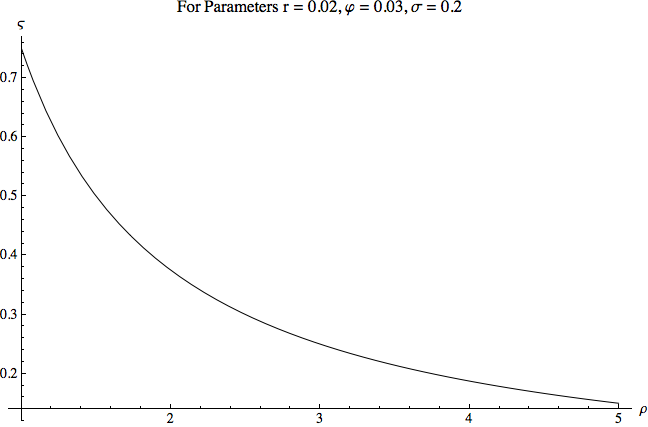
\includegraphics[width=6in]{./Figures/ShareVsCRRA}
  \end{figure}
  \begin{figure}
    \centering
    \caption{The Approximation Error for the Portfolio Share in Risky Assets $\riskyshare$ Is Small}
    \label{fig:Port:b}
    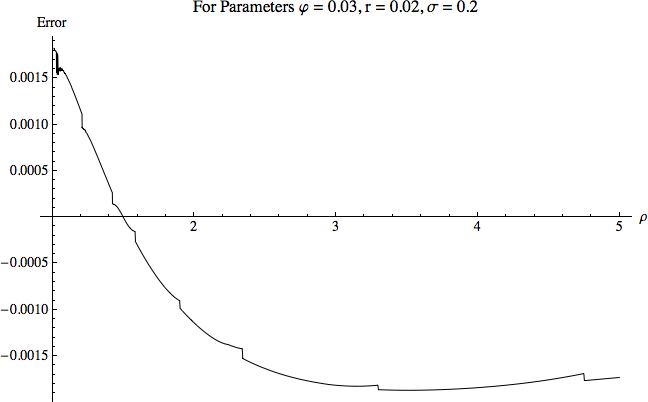
\includegraphics[width=6in]{./Figures/ShareApproxErr}
\begin{flushleft} \footnotesize Note: The approximation error is computed by solving for the exactly optimal
  portfolio share numerically.  See the \texttt{Portfolio-CRRA-Derivations.nb} Mathematica notebook for details.
  \end{flushleft}
\end{figure}

% Took a long time to figure out that something about the use of subfigures was causing the figures not to appear in html

% \begin{figure}[h]
% \caption{The Risky Portfolio Share $\riskyshare$ and Relative Risk Aversion $\CRRA$} \label{fig:Port}\centering
% \subfigure[The Approximate Risky Portfolio Share $\riskyshare$ Declines as Relative Risk Aversion $\CRRA$ Increases]{
%     \label{fig:Port:a}
%     \fbox{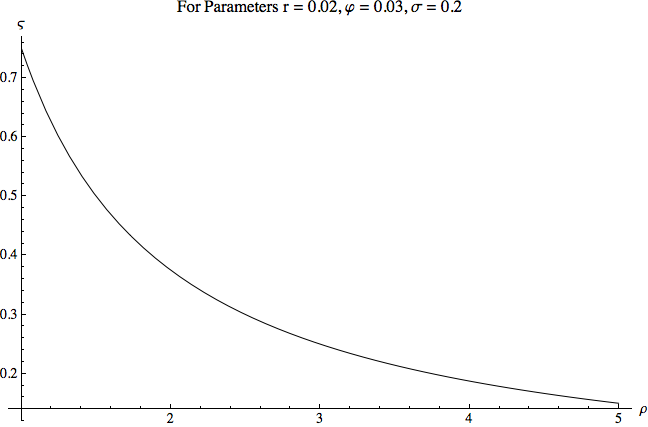
\includegraphics[width=6in]{./Figures/ShareVsCRRA}}
% }\\
% \vspace{.1in} \subfigure[The Approximation Error for the Portfolio Share in Risky Assets $\riskyshare$ Is Small] {
%     \label{fig:Port:b}
%     \fbox{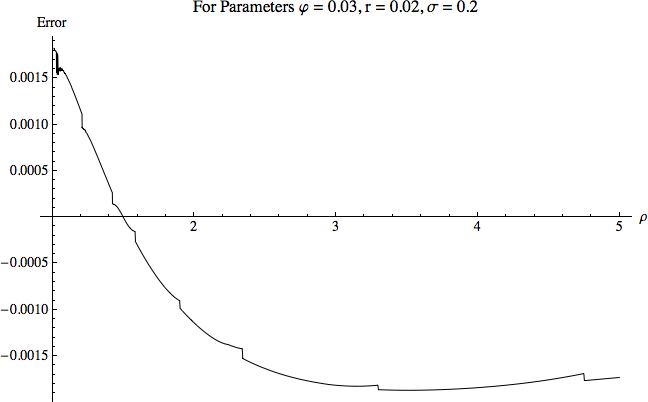
\includegraphics[width=6in]{./Figures/ShareApproxErr}}
% } \begin{flushleft} \footnotesize Note: The approximation error is computed by solving for the exactly optimal
% portfolio share numerically.  See the \texttt{Portfolio-CRRA-Derivations.nb} Mathematica notebook for details.
% \end{flushleft}
% \end{figure}

